\section{Weak Supervised Learning (WSL)}
\begin{frame}{}
    \LARGE Weak Supervised Learning (WSL)
\end{frame}

\begin{frame}[allowframebreaks]{}
    \begin{figure}
        \centering
        \fetchconvertimage{https://ai.stanford.edu/blog/assets/img/posts/2019-03-03-weak_supervision/dp.png}{images/contrastive/wsl-architecture.png}{height=0.9\textheight,width=1\textwidth,keepaspectratio}
    \end{figure}
\end{frame}

\begin{frame}[allowframebreaks]{What is Weak Supervised Learning?}
    \begin{itemize}
        \item Sometimes, we don't have perfect data or labels for training.
        \item \textbf{Weak Supervised Learning (WSL)} helps us learn even when our labels are not ideal.
        \item There are different ways labels can be "weak":
        \begin{itemize}
            \item \textbf{Incomplete labels:} Only some data points have labels.
            \item \textbf{Inexact labels:} Labels are not very detailed (e.g., we know what’s in an image, but not where).
            \item \textbf{Inaccurate labels:} Some labels might be wrong or noisy.
        \end{itemize}
    \end{itemize}

    \framebreak
    \begin{figure}
        \centering
        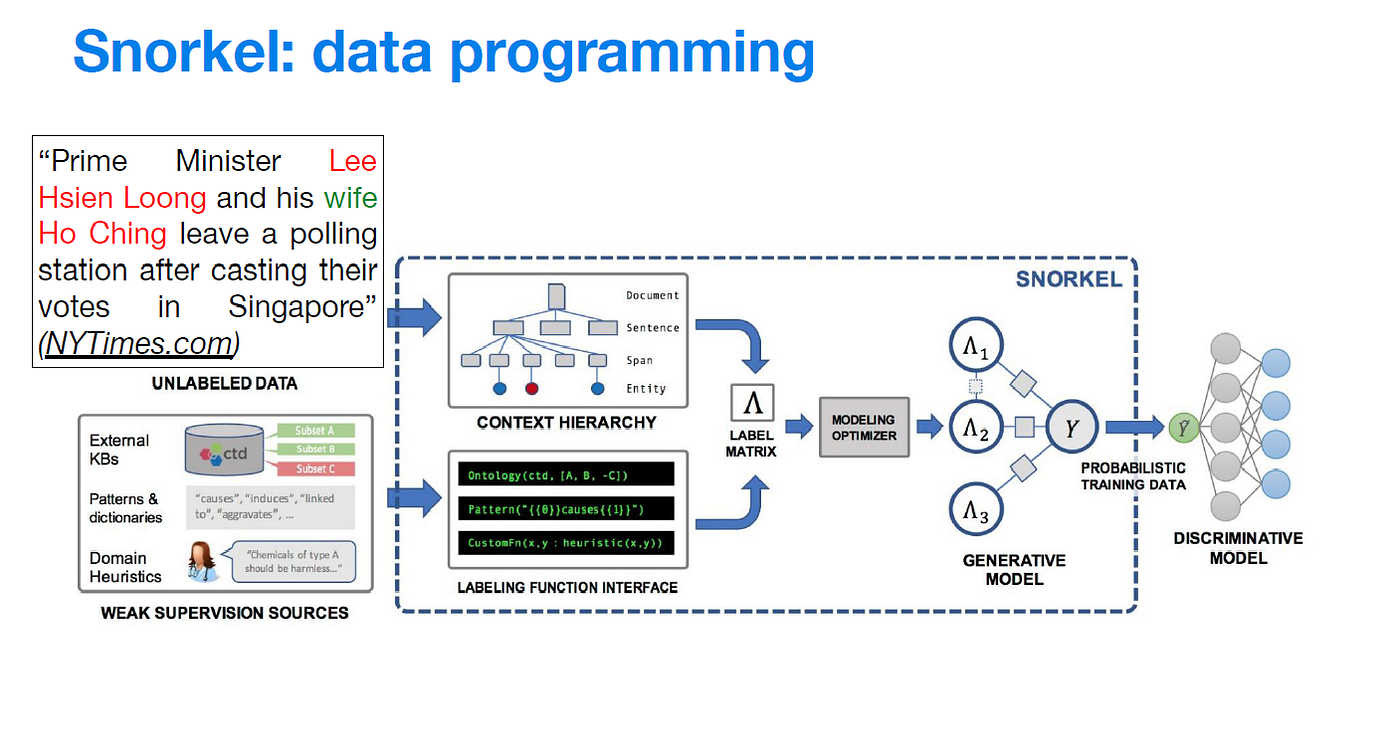
\includegraphics[width=1.05\linewidth,height=0.95\textheight,keepaspectratio]{images/contrastive/snorkel.png}
    \end{figure}

    \framebreak
    \textbf{Why do we use WSL?}
    \begin{itemize}
        \item Getting perfect labels for all data is expensive and slow.
        \item Experts are needed to label some data, which costs a lot.
        \item WSL lets us use cheaper, less perfect labels to train our models.
    \end{itemize}

    \framebreak
    \textbf{When is WSL useful?}
    \begin{itemize}
        \item When we have lots of data but not enough labels (like in medical images).
        \item When we can use rules or existing knowledge to help label data (like using a dictionary for text).
    \end{itemize}
\end{frame}

\begin{frame}[allowframebreaks]{WSL Taxonomy & Approaches}
    \begin{figure}
        \centering
        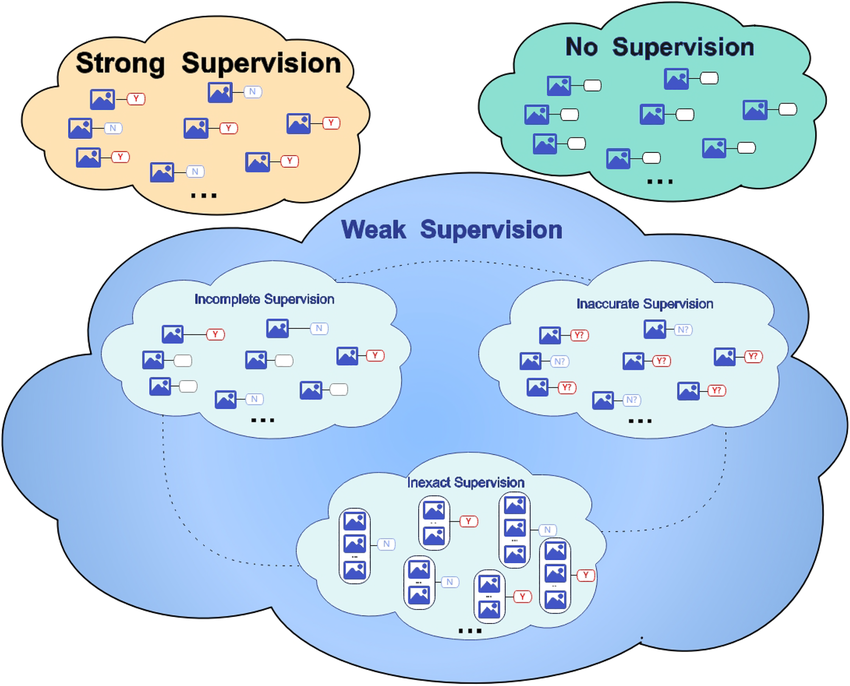
\includegraphics[width=\linewidth,height=0.9\textheight,keepaspectratio]{images/contrastive/weak-supervised.png}
    \end{figure}

    \framebreak
    \textbf{How can we do Weak Supervised Learning?}
    \begin{itemize}
        \item \textbf{Programmatic Labeling (Data Programming)}
        \begin{itemize}
            \item Write simple rules (labeling functions) to label data automatically.
            \item Use a tool like Snorkel to combine these noisy labels and clean them up.
            \item Steps: Unlabeled data $\rightarrow$ Rules $\rightarrow$ Cleaned labels $\rightarrow$ Train model.
            \item (Snorkel: Ratner et al., 2016)
        \end{itemize}
        \framebreak
        \item \textbf{Multiple Instance Learning (MIL)}
        \begin{itemize}
            \item Sometimes we only know if a group (bag) has something, not which item.
            \item Example: We know an image has a cat, but not where.
            \item The model learns to find the right items inside each group.
            \item Used in medical images, object detection, etc.
        \end{itemize}
        \framebreak
        \item \textbf{Webly / Noisy Label Learning}
        \begin{itemize}
            \item Get labels from the internet or crowdsourcing—they can be messy!
            \item Use special tricks to handle wrong or noisy labels (like Co-teaching).
        \end{itemize}
        \framebreak
        \item \textbf{Hybrid Methods (Semi + Weak Supervision)}
        \begin{itemize}
            \item Mix a small set of good labels with lots of weak ones.
            \item Use tricks like pseudo-labeling or learning in steps.
        \end{itemize}
    \end{itemize}
\end{frame}
